\documentclass[12pt]{kiarticle} % You can learn about my document class "kiarticle" and install it to your device by following the link: https://github.com/Kiarendil/toolkitex
%\graphicspath{{pictures/}}
\DeclareGraphicsExtensions{.pdf,.png,.jpg,.eps}
%%%
\usepackage{pgfplotstable}
\usepackage{graphicx}
\usepackage{pgf,tikz}
\usepackage{mathrsfs}
\usepackage{pgfplots}
\pgfplotsset{compat=1.9}
\usetikzlibrary{arrows}
\usetikzlibrary{shapes.geometric}
\usetikzlibrary{calc}
\pagestyle{fancy}
\fancyhf{}
%\renewcommand{\headrulewidth}{ 0.1mm }
\renewcommand{\footrulewidth}{ .0em }
\fancyfoot[C]{\texttt{\textemdash~\thepage~\textemdash}}
\fancyhead[L]{Лабораторная работа № 4.3.3 \hfil}
\fancyhead[R]{\hfil Иванов Кирилл, 625 группа }
\usepackage{multirow} % Слияние строк в таблице
\newcommand
{\un}[1]
{\ensuremath{\text{#1}}}
\newcommand{\eds}{\ensuremath{ \mathscr{E}}}
\usepackage{tikz}
%%% Работа с таблицами
\usepackage{array,tabularx,tabulary,booktabs} % Дополнительная работа с таблицами
\usepackage{longtable}  % Длинные таблицы
\usepackage{multirow} % Слияние строк в таблице
\newcommand{\specialcell}[2][c]{%
	\begin{tabular}[#1]{@{}c@{}}#2\end{tabular}}

\renewcommand{\thesubsection}{\arabic{subsection}}

\begin{document}
	
	\begin{titlepage}
		\begin{center}
			\large 	Московский физико-технический институт \\
			(государственный университет) \\
			Факультет общей и прикладной физики \\
			\vspace{0.2cm}
			
			\vspace{4.5cm}
			Лабораторная работа № 4.3.3 \\ \vspace{0.2cm}
			\large (Общая физика: оптика) \\ \vspace{0.2cm}
			\LARGE \textbf{Исследование разрешающей способности микроскопа методом Аббе}
		\end{center}
		\vspace{2.3cm} \large
		
		\begin{center}
			Работу выполнил: \\
			Иванов Кирилл,
			625 группа
			\vspace{10mm}		
			
		\end{center}
		
		\begin{center} \vspace{60mm}
			г. Долгопрудный \\
			2018 год
		\end{center}
	\end{titlepage}
	
	\paragraph*{Цель работы:} изучение дифракционного предела разрешения объектива микроскопа. 
	
	\paragraph*{Оборудование:} лазер, кассета с набором сеток разного периода, линзы, щель с микрометрическим винтом, экран, линейка. 
	
	\section{Теоретическое введение}
	
	Метод Аббе оценки разрешающей способности прибора основа на принципе Гюйгенса-Френеля: сначала рассматривается первичное изображение, или фурье-образ, предмета, получаемое в задней фокальной плоскости $F$ объектива; затем первичное изображение представляется источником волн, формирующих вторичное изображение в сопряженной плоскости $P_2$. Рисунок \ref{abbe} иллюстрирует образование изображения в объективе микроскопа. На рисунке $P_1$ - предметная плоскость. 
	
	\begin{figure}[h]
		\centering	
		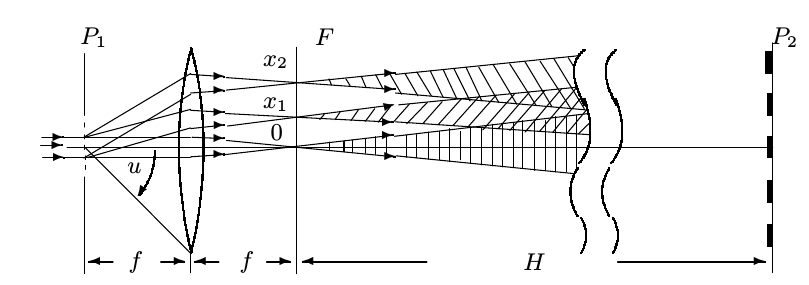
\includegraphics[width=0.6\textwidth]{abbe.png}
		\caption{Образование изображение в объективе микроскопа}
		\label{abbe}
	\end{figure}
	
	Первичное изображение является картиной дифракции Фраунгофера на объекте (в работе - на дифракционной решетке). Для одномерной решетки периода $d$ направление $\varphi_m$ на максимум интенсивности $x_m$ задается условием: 
	
	\begin{equation}
		d\sin\varphi_m = m\lambda
	\end{equation} 
	
	Здесь $\lambda$ - длина световой волны. 
	
	В плоскости $P_2$ наблюдается результат интерференции от когерентных точечных источников в $F$, создается изображение объекта. Согласно геометрической оптике, изображение в сопряженной плоскости имеет период: 
	
	\begin{equation}
		d' \approx \frac{H + f}{f} \cdot d = \Gamma d
	\end{equation}
	
	Здесь $\Gamma = \frac{H+f}{f}$ - увеличение, даваемое системой, соответствующие величины указаны на рисунке \ref{abbe}. 
	
	Для образование в $P_2$ периодичной структуры необходимо: $\varphi_m \le u$, где $u$ - апертурный угол. Откуда из формулы (1): 
	
	\[ \sin u \ge \lambda/d \]
	
	Обозначим диаметр рабочей части линзы объектива $D$, тогда $\sin u = \frac{D}{2f}$.
	
	Таким образом, оценено разрешимое объективом расстояние $d$:
	
	\begin{equation}
		d \ge \frac{\lambda}{\sin u} = \frac{2\lambda f}{D}
	\end{equation} 
	
	В работе используется двумерная дифракционная решетка, которую можно рассматривать как скрещенные одномерные. Контролируя размер диафрагмы, устанавливаемой в фурье-плоскости $F$, можно пропустить только вертикальные или горизонтальные максимумы и получить одномерное вторичное изображение. 
	
	
	\section{Определение периода решеток по их пространственному спектру}
	
	Схема установки, используемой в работе, изображена на рисунке \ref{shema}. Лазер светит перпендикулярно на двумерную решетку C (в кассете их 5 штук), расположенную вблизи фокальной плоскости длиннофокусной линзы $\text{Л}_1$. Вторичное изображение в плоскости $P_2$ проецируется на экран Э короткофокусной линзой $\text{Л}_2$. В фурье-плоскости $F$ ставится диафрагма диаметром $D$. Параметры установки: длина волны излучения лазера $\lambda = 532$ нм.
	
	\begin{figure}[h]
		\centering	
		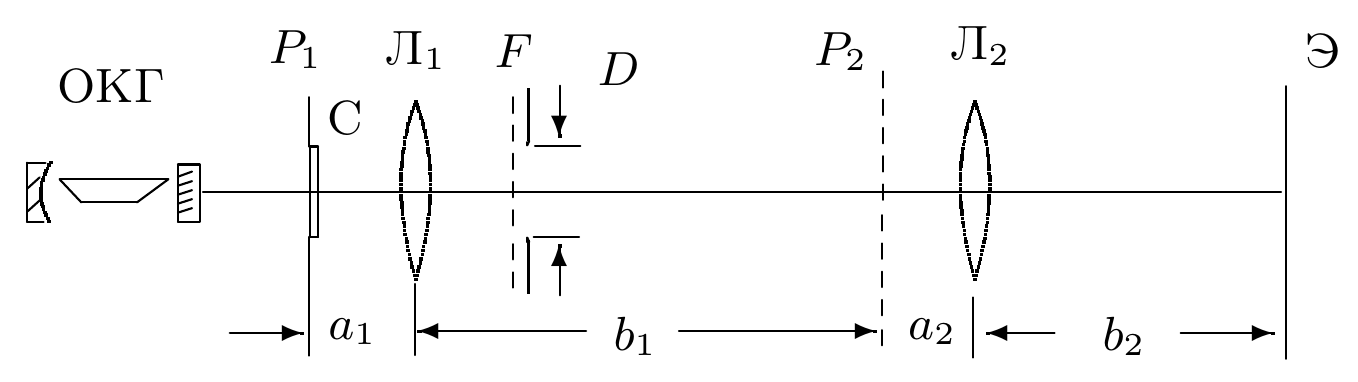
\includegraphics[width=0.7\textwidth]{shema.png}
		\caption{Схема экспериментальной установки - модель проекционного микроскопа}
		\label{shema}
	\end{figure}
	
	Для выполнения данного пункта частично соберем схему: установим на пути луча сетку и добьемся четкого изображения решеток на экране. Для увеличения точности измерений на миллиметровой бумаге отметим диапазон дифракционных максимумов для каждой сетки. Расстояние от сетки до экрана равно $L = (117,0 \pm 0,5)$ см. 
	
	По количеству отмеченных максимумов $m$ и их общей длине $l$ (ошибку примем равной 2 мм) определим период решеток $d$ из формулы (1). С учетом условия $\varphi = l/L$, получим:
	
	\[ d = \frac{(m-1)\lambda}{l/L} \]
	
	Вычисления содержатся в таблице \ref{period1}.
	
	\begin{table}[h]
		\centering
		\begin{tabular}{|c|c|c|c|c|}
\hline
№ решетки&$n$ &$l$, мм&$d$, мм&$\Delta d$, мм\\
\hline
1&25&94&0,159&0,004\\
\hline
2&22&111&0,118&0,002\\
\hline
3&15&147&0,0593&0,0010\\
\hline
4&9&161&0,0309&0,0005\\
\hline
5&7&187&0,0200&0,0003\\
\hline
\end{tabular}
		\caption{Измерение периода дифракционных решеток по их пространственному спектру}
		\label{period1}
	\end{table}	
	
	\section{Определение периода решеток по изображению, увеличенному при помощи модели микроскопа}
	
	Соберем модель проекционного микроскопа без диафрагмы в соответствии с изображенной на рисунке \ref{shema}; отцентрируем систему. Добьемся хорошей резкости картинки на экране для всех решеток. Измерим расстояния между сеткой и длиннофокусной линзой $\text{Л}_1$ $a_1 = (14,5 \pm 0,5)$ см, между короткофокусной линзой $\text{Л}_2$ $b_2 = (17,0 \pm 0,5)$ см и "длину тубуса" $\ b_1 + a_2 = (103,0 \pm 0,5)$ см (указаны на рисунке \ref{shema}). Расстояние $a_2$ приблизительно равно фокусному расстоянию линзы $\text{Л}_2$ и указано на установке $a_2 = 2,5$ см. Увеличение системы задается формулой: 
	
	\[ \Gamma = \frac{b_1b_2}{a_1a_2} = 47,1 \pm 1,3 \]
	
	Погрешность увеличения $\Gamma$ рассчитана в соответствии с правилом для погрешности произведения. 
	
	Как и в первой части работы, на миллиметровой бумаге отметим диапазон максимумов, наблюдаемых на экране для каждой решетки. Определим период изображения $d' = l/(m-1)$ и по формуле (2), где $\Gamma = (47,1 \pm 1,3)$, пересчитаем период решеток $d$. Вычисления содержатся в таблице \ref{period2}.
	
	\begin{table}[h]
		\centering
		\begin{tabular}{|c|c|c|c|c|c|c|c|c|c|c|}
\hline
№ решетки&$n$ &$l$, мм&$d'$, мм&$\Delta d'$, мм&$d$, мм&$\Delta d$, мм\\
\hline
1&10&87&9,7&0,2&0,205&0,007\\
\hline
2&13&87&7,25&0,17&0,154&0,005\\
\hline
3&22&70&3,33&0,10&0,071&0,003\\
\hline
4&27&44&1,69&0,08&0,036&0,002\\
\hline
5&28&30&1,11&0,07&0,024&0,002\\
\hline
\end{tabular}
		\caption{Измерение периода дифракционных решеток по изображению, увеличенному при помощи микроскопа}
		\label{period2}
	\end{table}	
	
	Измерения, выполненные в данном пункте, могут быть неточны, так как положение сетки лишь приближенно соответствует законам геометрической оптики. В кассете не было решетки с проволокой, по резкому изображению которой проводится правильная настройка. 
	
	\clearpage
	
	\section{Определение периода решеток по оценке разрешающей способности микроскопа}
	
	Поместим диафрагму в фокальную плоскость $F$, как это показано на рисунке \ref{shema}. Для каждой решетки определим минимальное размер щели $D_{min}$ (измеряется микрометрическим винтом с ошибкой 0,02 мм), при котором появляется двумерная структура, что соответствует открытию первых максимумов во втором направлении. 
	
	По формуле (3) при подстановке значения $D_{min}$ вычислим наименьшее разрешаемое микроскопом расстояние $d$ - период дифракционной решетки: 
	
	\[ d = \frac{2\lambda f}{D_{min}} \]
	
	Здесь $f$ - фокус линзы $\text{Л}_1$: $f = 110$ мм.  
	
	Вычисления содержатся в таблице \ref{period3}. 
	
	\begin{table}[h]
		\centering
		\begin{tabular}{|c|c|c|c|c|}
\hline
№ решетки&$D_{min}$, мм&$d$, мм&$\Delta d$, мм\\
\hline
1&0,57&0,205&0,007\\
\hline
2&0,76&0,154&0,004\\
\hline
3&1,15&0,102&0,002\\
\hline
\end{tabular}
		\caption{Измерение периода дифракционных решеток по оценке разрешающей способности микроскопа}
		\label{period3}
	\end{table}	
	
	Определить положение щели, при котором наблюдается двумерная структура, для решеток с меньшим периодом (№ 4, 5) не удалось: при максимальном открытии диафрагмы оставалось изображение одномерной сетки. 
	
	Измерения, приведенные в графе $D_{min}$, могут быть сдвинуты на несколько десятых миллиметра: микрометрический винт прокручивался при закрытой щели в сторону уменьшения.
	
	\
		
	Проверим теорию Аббе. Для этого построим график зависимости $d(1/D_{min})$, где значения $d$ возьмем из первой части работы (определенные по спектру). Необходимые величины сведены в таблицу \ref{dD}. 
	
	\begin{table}[h]
		\centering
		\begin{tabular}{|c|c|c|c|c|c|c|}
\hline
$1/D_{min}$, $\text{мм}^{-1}$&1,75&1,32&0,870\\
\hline
$\Delta 1/D_{min}$, $\text{мм}^{-1}$&0,06&0,03&0,015\\
\hline
$d$,мм&0,159&0,118&0,0593\\
\hline
$\Delta d$, мм&0,004&0,002&0,0010\\
\hline
\end{tabular}
		\caption{Измерение зависимости периода решетки d (взят по спектру) от размера щели $D_{min}$, при котором проявляется двумерная структура}
		\label{dD}
	\end{table}	
	
	По таблице \ref{dD} построен график зависимости $d(1/D_{min})$, изображенный на рисунке \ref{oops}. Экспериментальные точки, как того и требует теоретическая зависимость (8), ложатся на прямую с хорошей точностью. Величина наклона прямой и ошибка, определенная по методу $\chi^2$, отражены на графике. Ошибка составляет 7\%. В пределах погрешности значение коэффициента наклона совпадает с теоретическим $b = 2\lambda f \approx 0,117 \text{ мм}^2$.
	
	\begin{figure}[h]
		\centering
		
		\pgfplotstableread {
			x			y			xerr		yerr
			1.75		0.159		0.06		0.004
			1.32		0.118		0.03		0.002
			0.870		0.0593		0.015		0.0010
		}\datatable
		\pgfplotstablecreatecol[linear regression={y=y}]{regression}{\datatable}
		\xdef\coefA{\pgfplotstableregressiona} % save the slope parameter
		\xdef\coefB{\pgfplotstableregressionb} % save the intercept parameter
		
		\begin{tikzpicture}
		
		\begin{axis}[width = 0.6\textwidth, 
		%axis lines = middle,
		%axis line style = thick,
		xlabel = {$1/D_{min}$, $\text{мм}^{-1}$},
		ylabel = {$d$, мм}
		%every axis x label/.style={at={(current axis.right of origin)},anchor=north west},
		%every axis y label/.style={at={(current axis.above origin)},anchor=north east},	
		]
		
		\addplot[only marks,
		mark size=1,
		black,
		error bars/.cd,
		x dir = both, x explicit,
		y dir = both, y explicit,
		] table
		[x=x, y=y, x error = xerr, y error = yerr ]
		{	
			x			y			xerr		yerr
			1.75		0.159		0.06		0.004
			1.32		0.118		0.03		0.002
			0.870		0.0593		0.015		0.0010
		};
		
		%\addplot [thick, no markers, domain=1.3:3.5] {\coefB + \coefA*x};
		\addplot [thick, no markers, domain=0.85:1.85] {-0.046 + 0.121*x};
		
		\node at (700, 10) {\begin{tabular}{c} $d = b/D + a$ \\ $b = (0,121 \pm 0,008) \text{ мм}^{2}$  \end{tabular}};
		\end{axis}
		\end{tikzpicture}
		\caption{График зависимости периода решетки, взятого по спектру, от диаметра диафрагмы $d(1/D_{min})$}
		\label{oops}
	\end{figure}
	
	\section{Наблюдение пространственной фильтрации и мультиплицирования}
	
	В этой части работы будем работать с решеткой №2.
	
	Максимумы, создаваемые двумерной решеткой в фокальной плоскости объектива $F$ (см. рисунок \ref{abbe}), представляют картину дифракции Фраунгофера и будут рассмотрены как первичное изображение. Они изображены на рисунке \ref{2d}.
	
	\begin{figure}[h]
		\centering	
		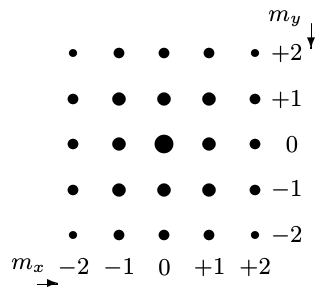
\includegraphics[width=0.3\textwidth]{2d.png}
		\caption{Дифракция Фраунгофера на двумерной решетке}
		\label{2d}
	\end{figure}
	
	Отфильтруем максимумы в одном из направлений решетки. Для этого подберем ширину щели таким образом, чтобы она пропускала только максимум нулевого порядка в перпендикулярном направлении. Поворачивая щель относительно оси системы, пронаблюдаем, как изменяется картина на экране, демонстрируя \textbf{пространственную фильтрацию}. 
	
	При вертикальной щели пропускаются максимумы $(0, m_x)$, и на экране наблюдается вертикальная "полоса" \ размытых максимумов. При горизонтальной щели, наоборот, пропускаются максимумы $(m_y, 0)$, и на экране видна горизонтальная "полоса". При положении щели под углом $45^\circ$ к вертикали наблюдается полоса максимумов $m_x = m_y$. Фотографии эффекта приведены на рисунке \ref{rotate}. 
	
	\begin{figure}[h]
		\begin{minipage}[h]{0.3\linewidth}
			\center{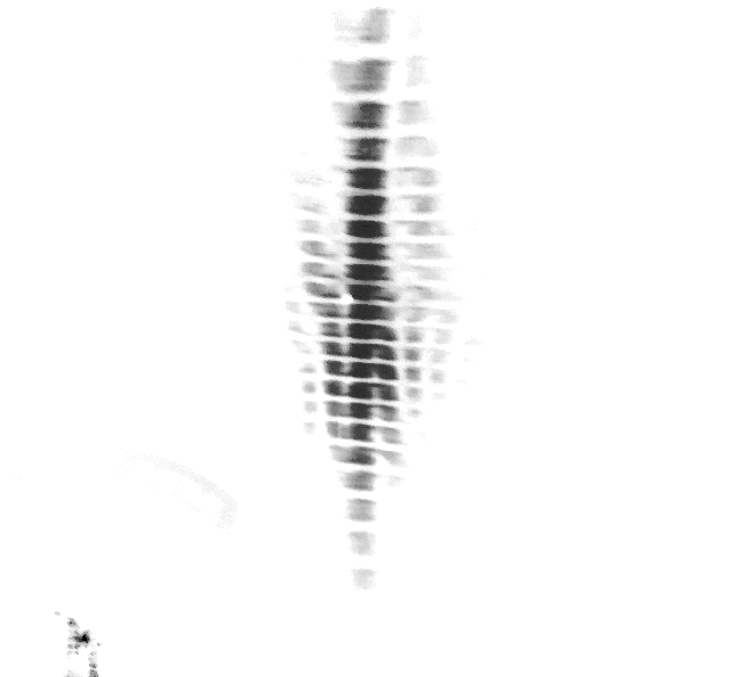
\includegraphics[width=0.9\linewidth]{vert.png} \\ a)}
		\end{minipage}
		\hfill
		\begin{minipage}[h]{0.3\linewidth}
			\center{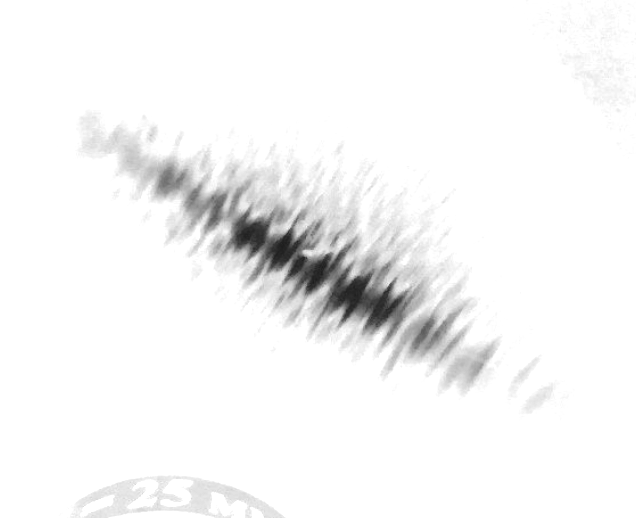
\includegraphics[width=0.9\linewidth]{mid.png} \\ b)}
		\end{minipage}
		\hfill
		\begin{minipage}[h]{0.3\linewidth}
			\center{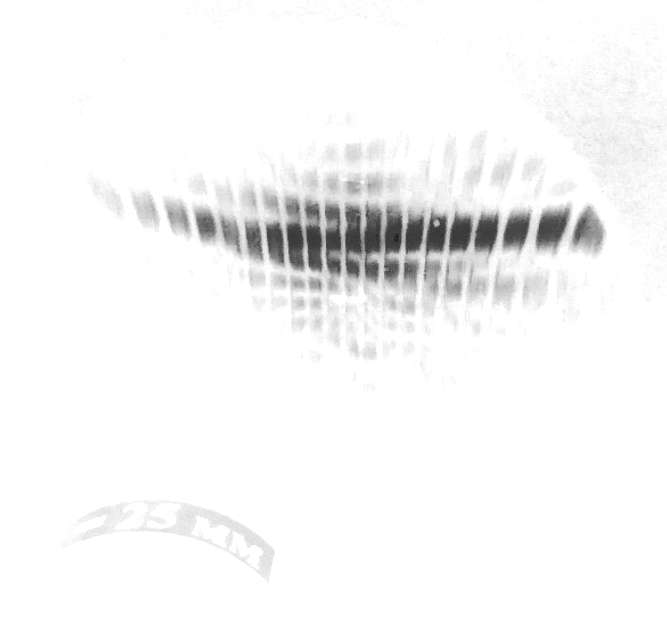
\includegraphics[width=0.9\linewidth]{hor.png} \\ c)}
		\end{minipage}
		\caption{Наблюдаемая картинка пространственной фильтрации: (a) при вертикальной щели, (b) при наклонной на $45^\circ$ щели, (c) горизонтальной щели }
		\label{rotate}
	\end{figure}

	\begin{figure}[h!]
	\centering	
	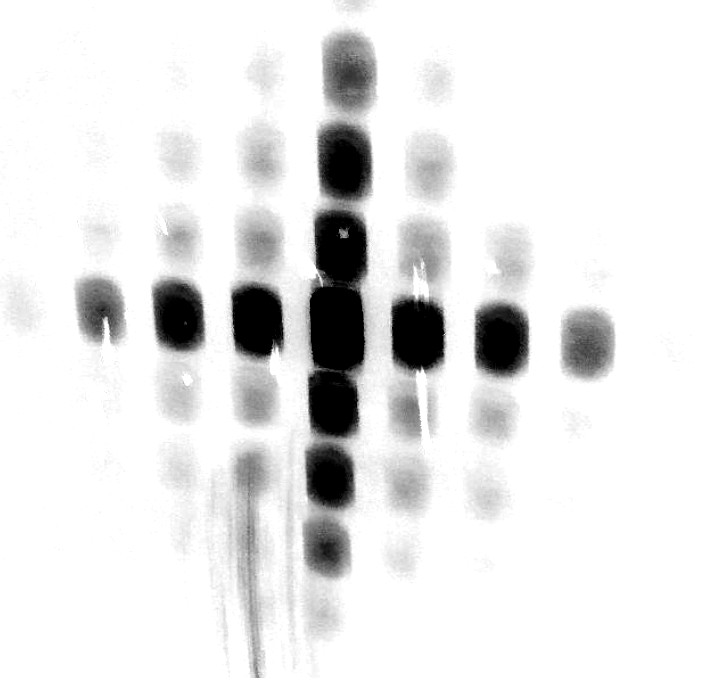
\includegraphics[width=0.4\textwidth]{mult.png}
	\caption{Наблюдаемая картина при мультиплицировании}
	\label{mult}
\end{figure}
	
	Нечеткость изображения можно объяснить наличием длинного козырька на подставке с сетками, способного изменить угол падения лучей на решетку.
	
	Далее пронаблюдаем \textbf{мультиплицирование}. Для этого поменяем местами диафрагму с узкой щелью и решетку местами. Тогда в фокальной плоскости $F$ получим результат дифракции на щели, а решетка рассечет это первичное изображение. Наблюдаемая картинка запечатлена на фотографии на рисунке \ref{mult}. 


\section{Вывод} 

В работе определены периоды исследуемых решеток тремя методами: по пространственному спектру, по увеличенному микроскопом изображению и по оценке разрешающей способности микроскопа (указаны в таблицах \ref{period1}-\ref{period3}). Полученные значения изменяются в пределах 20\%. Более достоверными являются измерения в первой части работы (по спектру), так как они в меньшей степени зависят от качества установки и настройки системы. 

Проверена теория Аббе разрешающей способности микроскопа, для чего построен график зависимости $d(1/D_{min})$, теоретически являющейся линейной. Действительно, экспериментальные точки хорошо легли на прямую, и коэффициент ее наклона, определенный по графику $b_{exp} = (0,121 \pm 0,008) \text{ мм}^2$ соотносится с теоретической константой $b_{theor} \approx 0,117$, что подтверждает состоятельность метода Аббе.

Изучены эффекты пространственной фильтрации и мультиплицирования.  
	
\end{document}